\documentclass[11pt]{article}
\usepackage[margin=1in]{geometry}
\usepackage{graphicx}
\usepackage{booktabs}
\usepackage{amsmath}
\usepackage{siunitx}
\usepackage{caption}
\usepackage[table]{xcolor}
\usepackage{titlesec}
\usepackage[hidelinks]{hyperref}
\titlespacing*{\section}{0pt}{6pt}{2pt}
\titlespacing*{\subsection}{0pt}{4pt}{1pt}
\captionsetup{font=small,labelfont=bf,skip=2pt}
\setlength{\parskip}{4pt}
\setlength{\parindent}{0pt}

\begin{document}

\begin{center}
{\large\bfseries Art as an Investment: A Hedge That Isn't}\\[2pt]
{\small FA26\_FIN\_680\_3238 --- Case 1 \quad|\quad Investment Committee Memorandum \quad|\quad Sep 21, 2026}\\[2pt]
{\small\itshape Managing Partner: [MD] \quad Analysts: [Name], [Name] \quad Client persona: UHNW single-family office}
\end{center}
\vspace{-4pt}
\hrule
\vspace{6pt}

\section*{Recommendation}
\textbf{Do not allocate to art as a portfolio hedge.} We tested the two claims that could justify a
seat for art in a family-office portfolio --- that it hedges inflation and that it cushions market
shocks --- against 46 years of quarterly index data (Bloomberg ARTDAI, 1980--2026). Both fail. Art
returned \textbf{4.1\% nominal (\(\approx\)1\% real) per year} versus \(\approx\)11\% for the S\&P~500,
its purchasing power \emph{falls} when inflation rises, it dropped 25--56\% in every major crisis with
5--16 year recoveries, and at a realistic 4\% weight it changes a 60/40 portfolio by less than
0.2~percentage points on any axis. The only defensible allocation is \textbf{$\le$2\%, and only as a
consumption/prestige asset held 10+ years --- never underwritten as a hedge.}

\section{The opportunity, and why it is tempting}
The pitch is real. Blue-chip art has a low \emph{reported} correlation to equities, a multi-decade
uptrend, a growing financialization ecosystem (Sotheby's Financial Services' \$12B+ loan book, a
\$700M art-backed securitization in 2024, a resurgence of art funds), and a demand tailwind from
rising UHNW wealth. British Rail's pension fund famously used art to beat 1970s inflation. If art
truly diversified and hedged inflation, a family office --- long horizon, tolerant of illiquidity ---
is exactly the holder who could harvest that premium. That is the bull case we set out to verify, not
to assume. The evidence, not the conclusion, leads what follows.

\section{Test 1 --- Inflation hedge: rejected}
If art hedged inflation, its nominal return would rise roughly one-for-one with CPI. It does not.
Regressing quarterly nominal art returns on realized inflation (controlling for the equity market,
Newey--West standard errors) gives an inflation beta of \textbf{$-0.06$} (t~$=-0.18$); full pass-through
($\beta=1$) is \textbf{rejected at p~$=0.001$}. Adding market-implied expected inflation (breakevens,
2003+) leaves the beta near zero (0.04). Most damning, art's \emph{real} return falls as inflation
rises: a real-return-on-inflation beta of \textbf{$-1.01$} (t~$=-2.97$). The British Rail story was a
1970s artifact; in the modern regime art behaves like a long-duration risk asset that is \emph{hurt}
by the rising rates that accompany inflation --- which is exactly what happened in 2022, when art fell
25\% during the inflation shock (Exhibit~2).

\section{Test 2 --- Diversification and crash protection: weak and unreliable}
On returns (not price levels), art's correlation to the S\&P~500 is \textbf{0.19} --- low, but the
widely cited ``0.88'' or ``0.62'' figure is a \textbf{spurious levels correlation} of two trending
series and should be disregarded (Exhibit~1). A 4\% art sleeve lowers in-sample 60/40 variance by only
4\%. The problem is that this modest benefit \emph{disappears when it is needed}: in modern crises the
art--equity correlation \textbf{rises to 0.30, versus 0.10 in calm quarters} (Exhibit~3), and the
five-year rolling correlation reached 0.61 in 2008. Art did not protect capital in any recent shock:
$-35\%$ in the GFC (still below its 2008 peak today), $-25\%$ in 2022 (also unrecovered), and even in
the mild COVID episode it fell 15\%. It fell \emph{less} than equities in 2008 only because auction
prices are sticky --- a reporting lag, not a hedge.

\section{The hidden risks the averages conceal}
\textbf{Smoothing cuts the other way than expected (Exhibit~5).} The standard critique is that
appraisal smoothing inflates Sharpe ratios and hides volatility. Our index shows the opposite: a
\emph{negative} first-order autocorrelation of $-0.62$, i.e.\ noise and mean reversion, not positive
smoothing. Either way there is no free lunch --- raw quarterly volatility is a high 31\% (annualized),
the CAPM beta is 0.22--0.37 with an \emph{insignificant, slightly negative} alpha, and part of the
``low correlation'' is simply measurement noise that biases correlation toward zero.

\textbf{The tail is a crowded trade (Exhibit~4).} The 1980s Japanese bubble is the cleanest warning.
As Japanese capital concentrated in one segment, prices ran up several-fold, then the broad index fell
\textbf{56\%}, Impressionist/Modern \textbf{65\%}, and the top ``Tier One'' names \textbf{88\%}, with
10--16 year recoveries. The crash \emph{scaled with prestige}: the ``blue-chip'' art sold as the safe
choice was the most fragile. A single marginal buyer made and unmade the market. Any index that begins
in 2000 cannot see this episode at all --- the exact ``black-swan correlation hidden by short or
smoothed indices'' the committee should fear. Our 1980-start data makes it visible; most published
art-fund track records do not.

\textbf{Illiquidity and cost are unmodeled and adverse.} Recovery periods of a decade-plus, no interim
marks, and \(\approx\)25\% round-trip auction friction (plus insurance and storage) all sit outside
the return figures above and make every result worse in practice.

\section{Opportunity cost --- what art actually does to the portfolio}
This is the decisive test for a family office. Overlaying a 4\% art sleeve on a 60/40 (2002--2026)
changes annual return by \textbf{$-0.09$~pp}, volatility by \textbf{$-0.19$~pp}, and maximum drawdown
by \textbf{$+0.1$~pp} --- Sharpe is unchanged at 0.86 (Table~1). In the 2022 inflation drawdown the art
sleeve improved the portfolio by 0.1~pp. Art is, at a realistic weight, a \textbf{do-nothing
allocation}: the theoretical diversification is too small to matter, and it is purchased with real
illiquidity and cost. The opportunity cost of the capital --- left in the 60/40 or in equities --- is
the entire case against.

\begin{table}[h]
\centering
\caption{60/40 with vs.\ without an art sleeve (quarterly, 2002Q4--2026Q2).}
\small
\begin{tabular}{lcccc}
\toprule
Portfolio & Ann.\ return & Ann.\ vol & Sharpe & Max drawdown \\
\midrule
60/40 (base) & 7.64\% & 8.85\% & 0.86 & $-24.8\%$ \\
59/39/2 art & 7.60\% & 8.75\% & 0.87 & $-24.8\%$ \\
58/38/4 art & 7.55\% & 8.66\% & 0.87 & $-24.9\%$ \\
\bottomrule
\end{tabular}
\end{table}

\section{Decision, sizing, and how we would (not) invest}
\textbf{As a hedge or return engine: no allocation.} Art fails the inflation test, fails the shock
test, adds nothing to the portfolio at a realistic weight, and hides a crowded-trade tail. If the
family's non-financial goals (enjoyment, legacy, philanthropy, collector identity) genuinely warrant
it, we would cap exposure at \textbf{2\% of investable assets}, treat any return as incidental, insist
on a \textbf{10+ year horizon}, and access it through a \textbf{diversified, moderate-fee fund or
lending strategy} --- never single trophy works (idiosyncratic, illiquid) and never high-fee retail
fractional platforms whose costs consume the thin returns. The honest alternative for the hedging
mandate is conventional: TIPS and short-duration bonds for inflation, quality and trend for shocks.

\textbf{Would our personal decision differ?} Marginally, and only in \emph{kind}. As individuals we
would buy a painting we love and never call it an investment; the analysis simply confirms that the
financial return is not the reason to own it. For the client's balance sheet, the committee's decision
and our personal decision converge: decline.

\section*{Limitations}
Results use one broad auction index (repeat-sale, still an approximation of an untradeable collection);
the requested long gold series failed to download and is omitted rather than proxied; the 60/40 overlay
is constrained to 2002+ by bond-ETF history; and desmoothing is model-dependent. None of these
plausibly reverse the conclusion --- the failures are large, consistent across four independent tests,
and directionally robust.

\vfill

% ---------------- EXHIBITS ----------------
\clearpage
\section*{Exhibits}

\begin{figure}[h]\centering
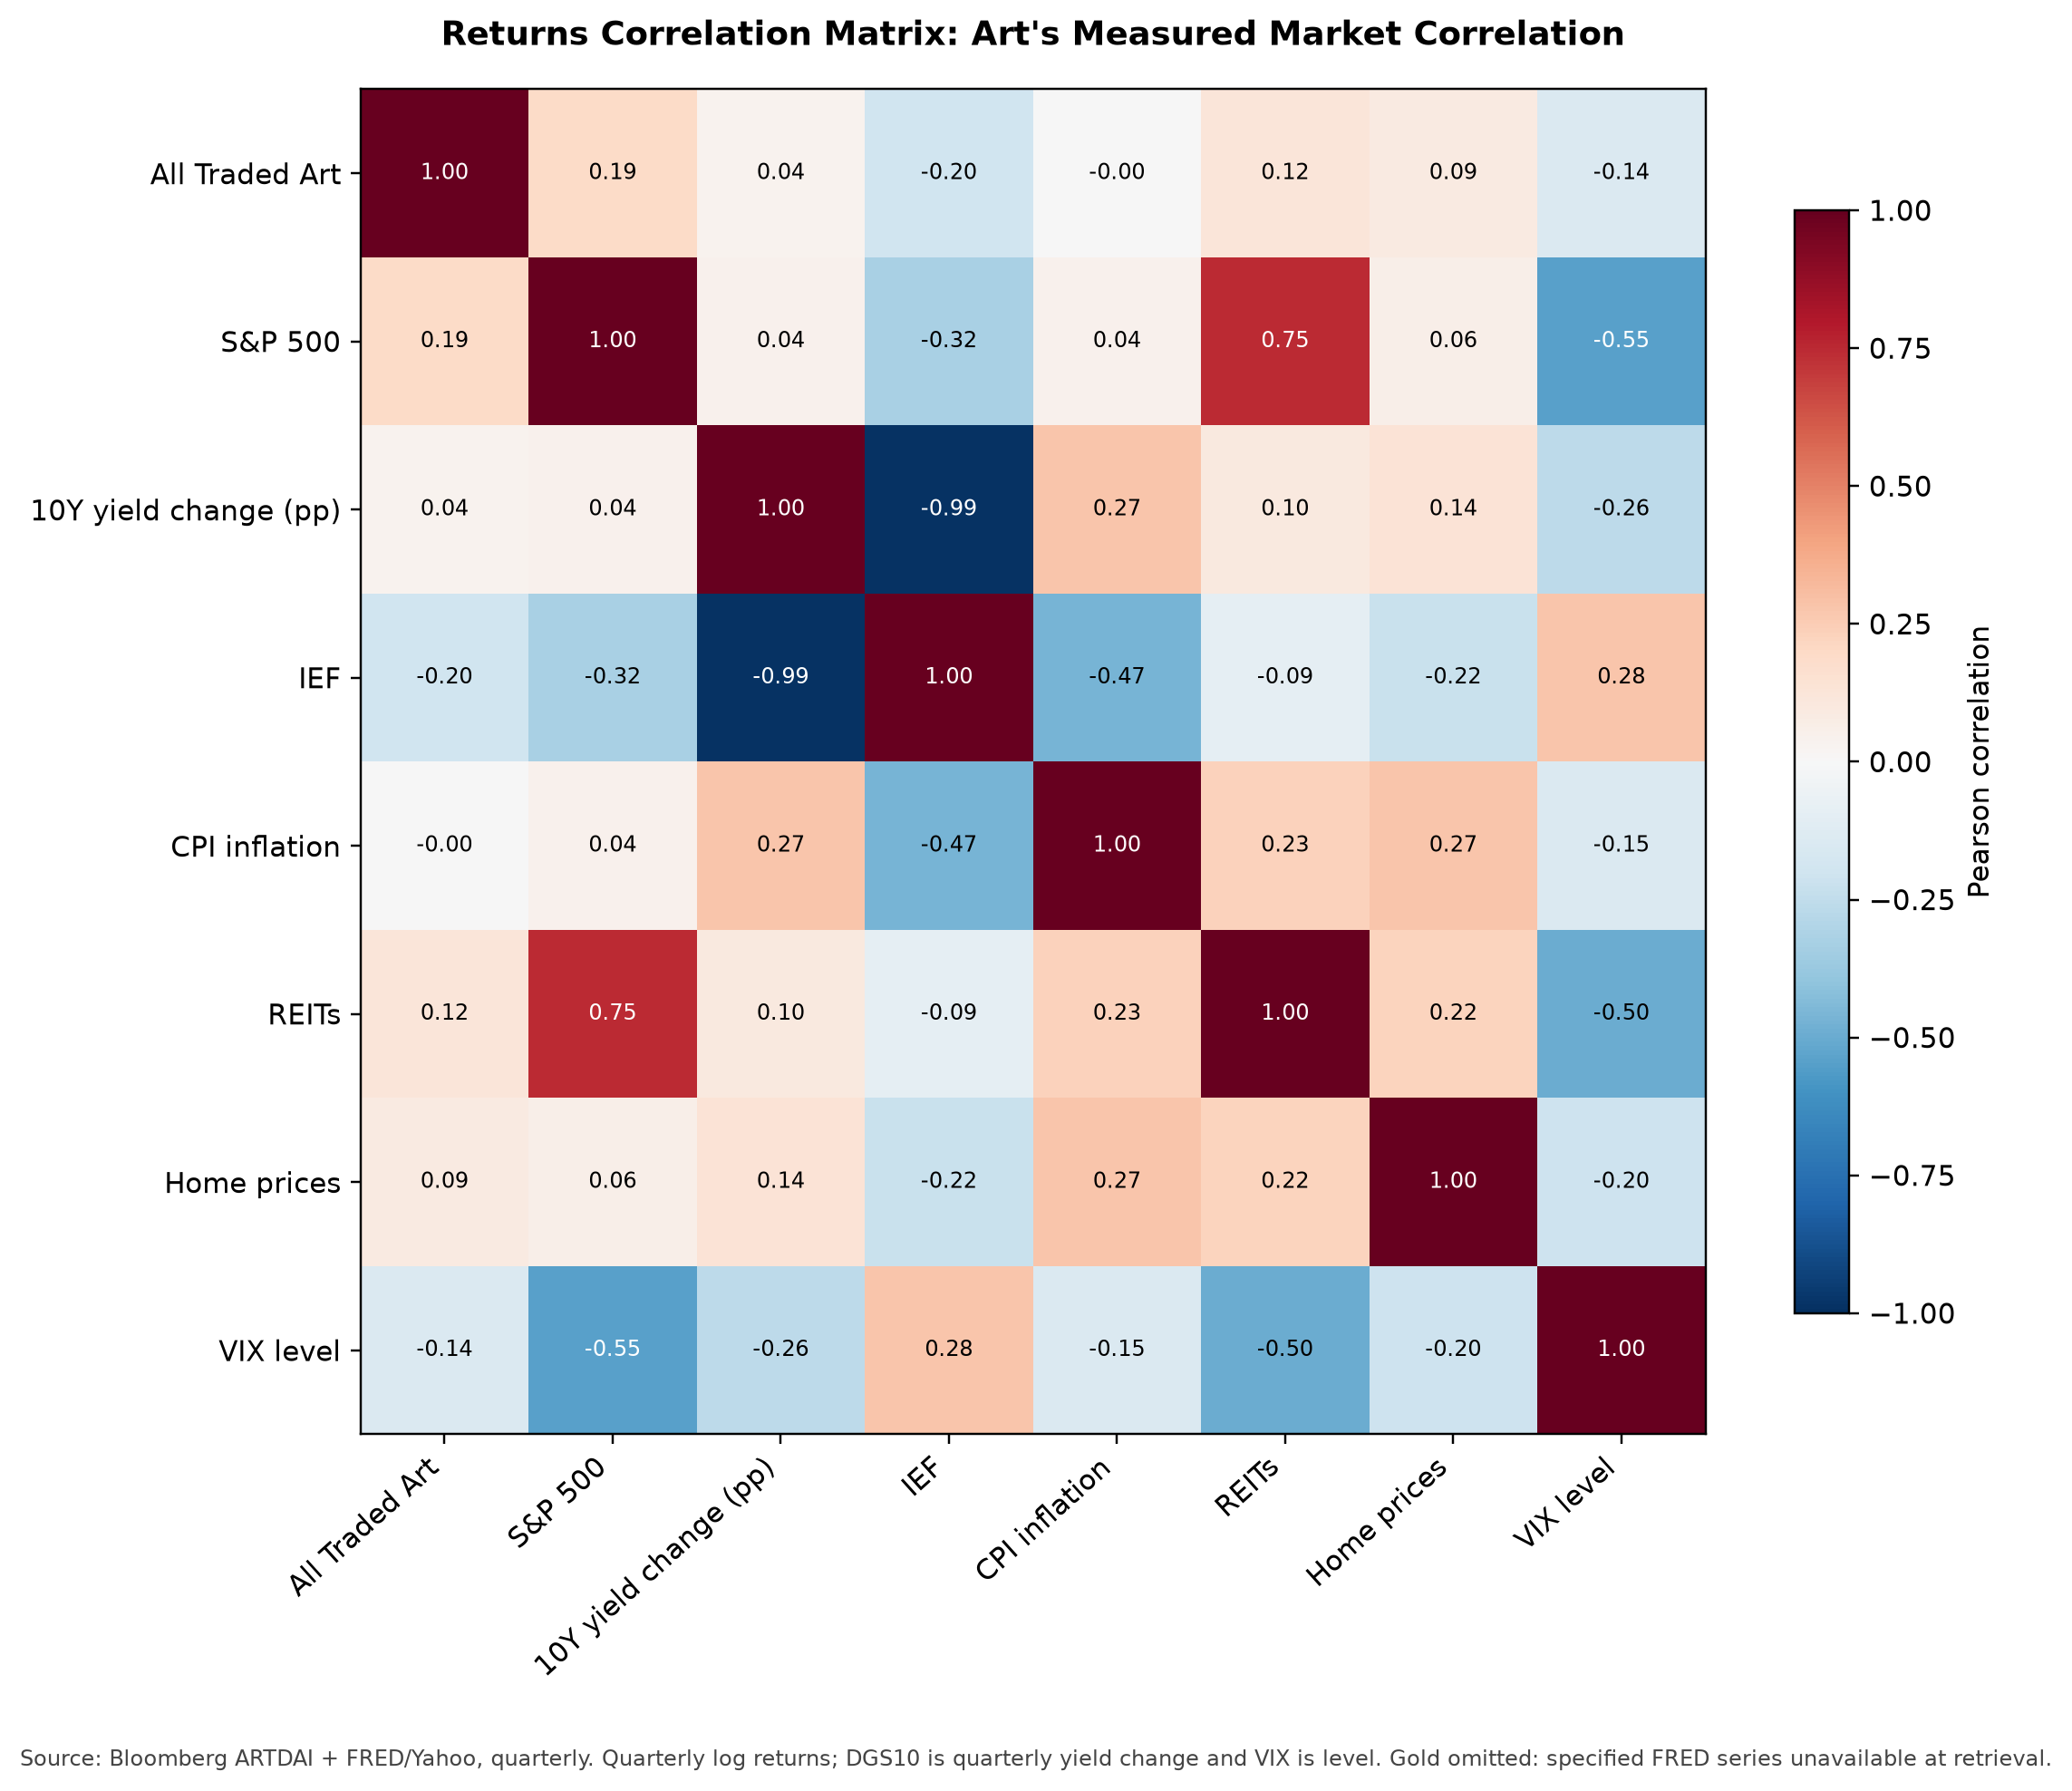
\includegraphics[width=0.72\textwidth]{exhibits/ex1_corr_heatmap.png}
\caption{Return correlations across assets (quarterly log returns, 1980--2026). Art's correlation to
the S\&P is 0.19 on returns vs.\ 0.62 on price levels (spurious). Source: Bloomberg ARTDAI + FRED/Yahoo.}
\end{figure}

\begin{figure}[h]\centering
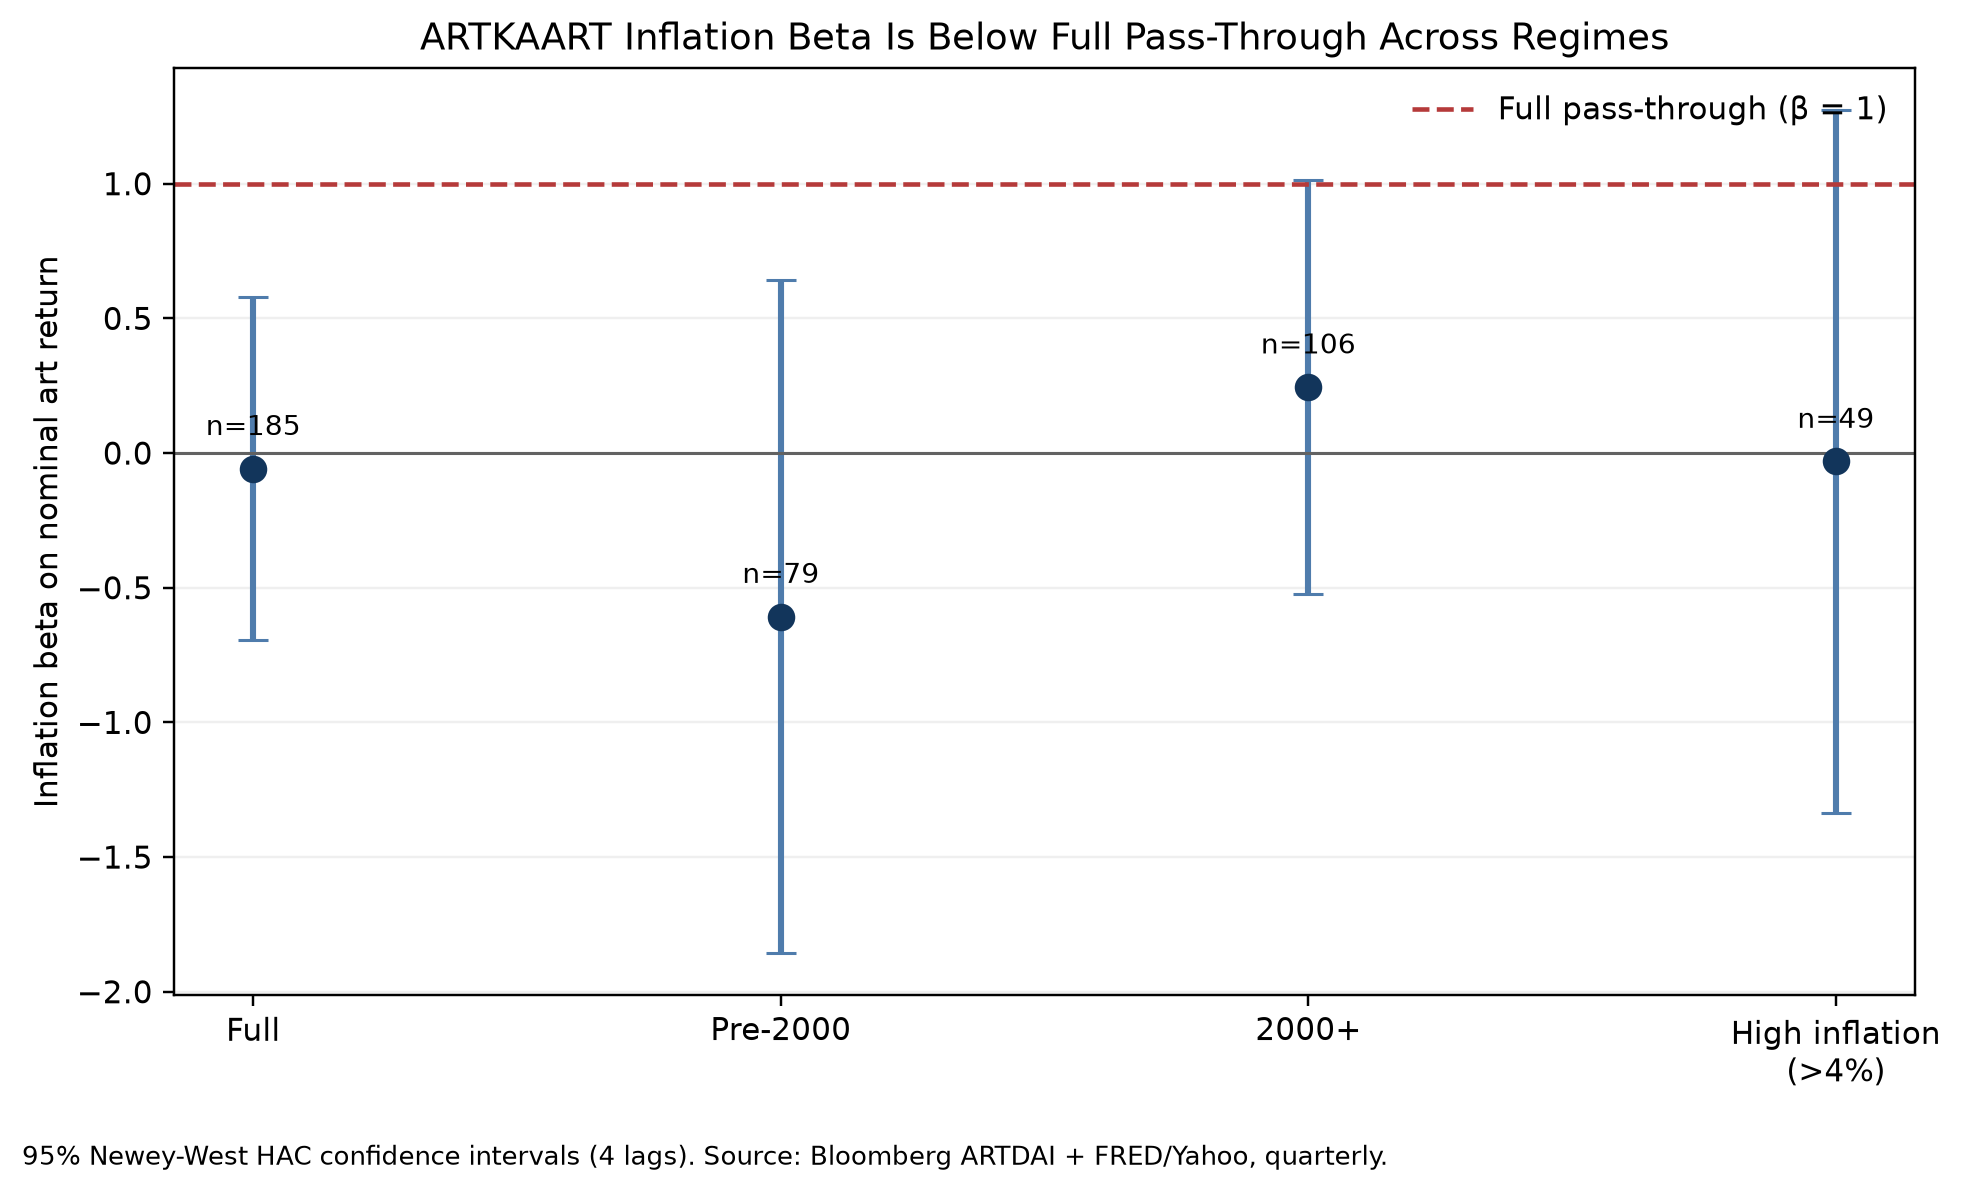
\includegraphics[width=0.72\textwidth]{exhibits/ex2_inflation_beta.png}
\caption{Inflation beta of art returns across regimes with HAC confidence bars. No specification shows
the one-for-one pass-through an inflation hedge requires. Source: Bloomberg ARTDAI + FRED.}
\end{figure}

\clearpage
\begin{figure}[h]\centering
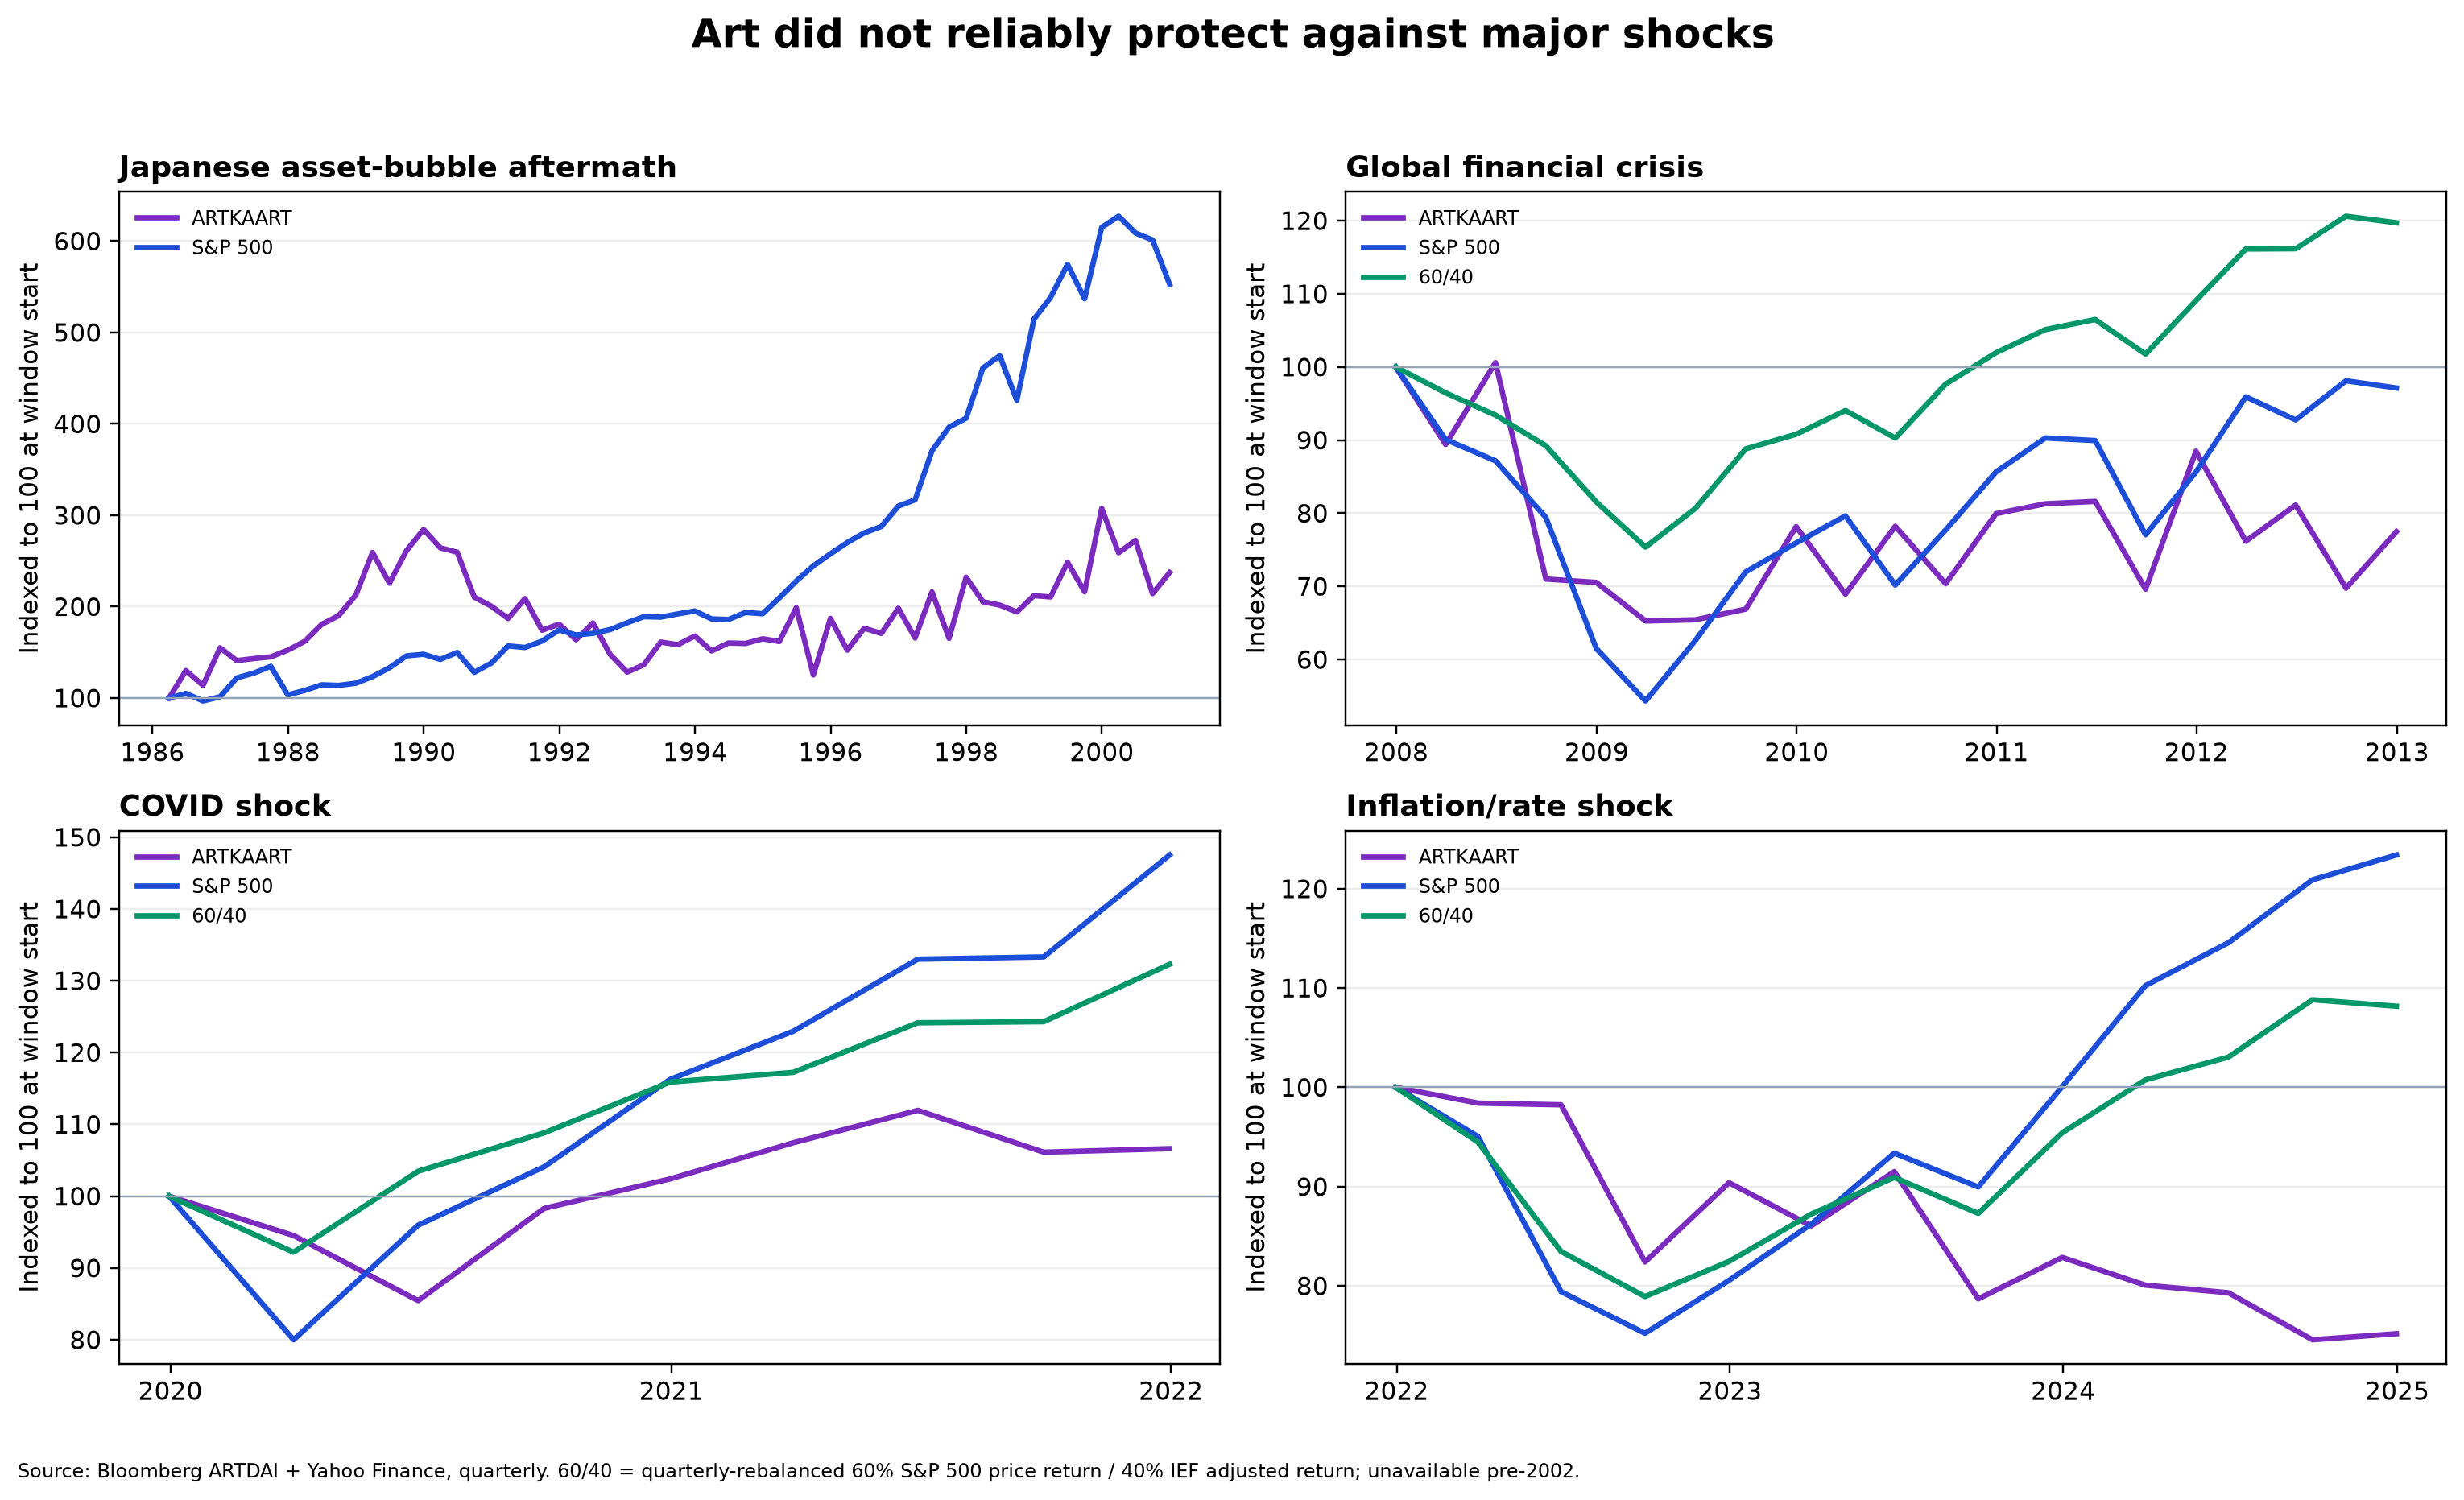
\includegraphics[width=0.86\textwidth]{exhibits/ex3_crisis_drawdowns.png}
\caption{Art vs.\ S\&P vs.\ 60/40 through four crises. Art suffered 15--56\% drawdowns with slow or no
recovery, and its correlation to equities rose in modern crises (0.30 vs.\ 0.10 calm).}
\end{figure}

\begin{figure}[h]\centering
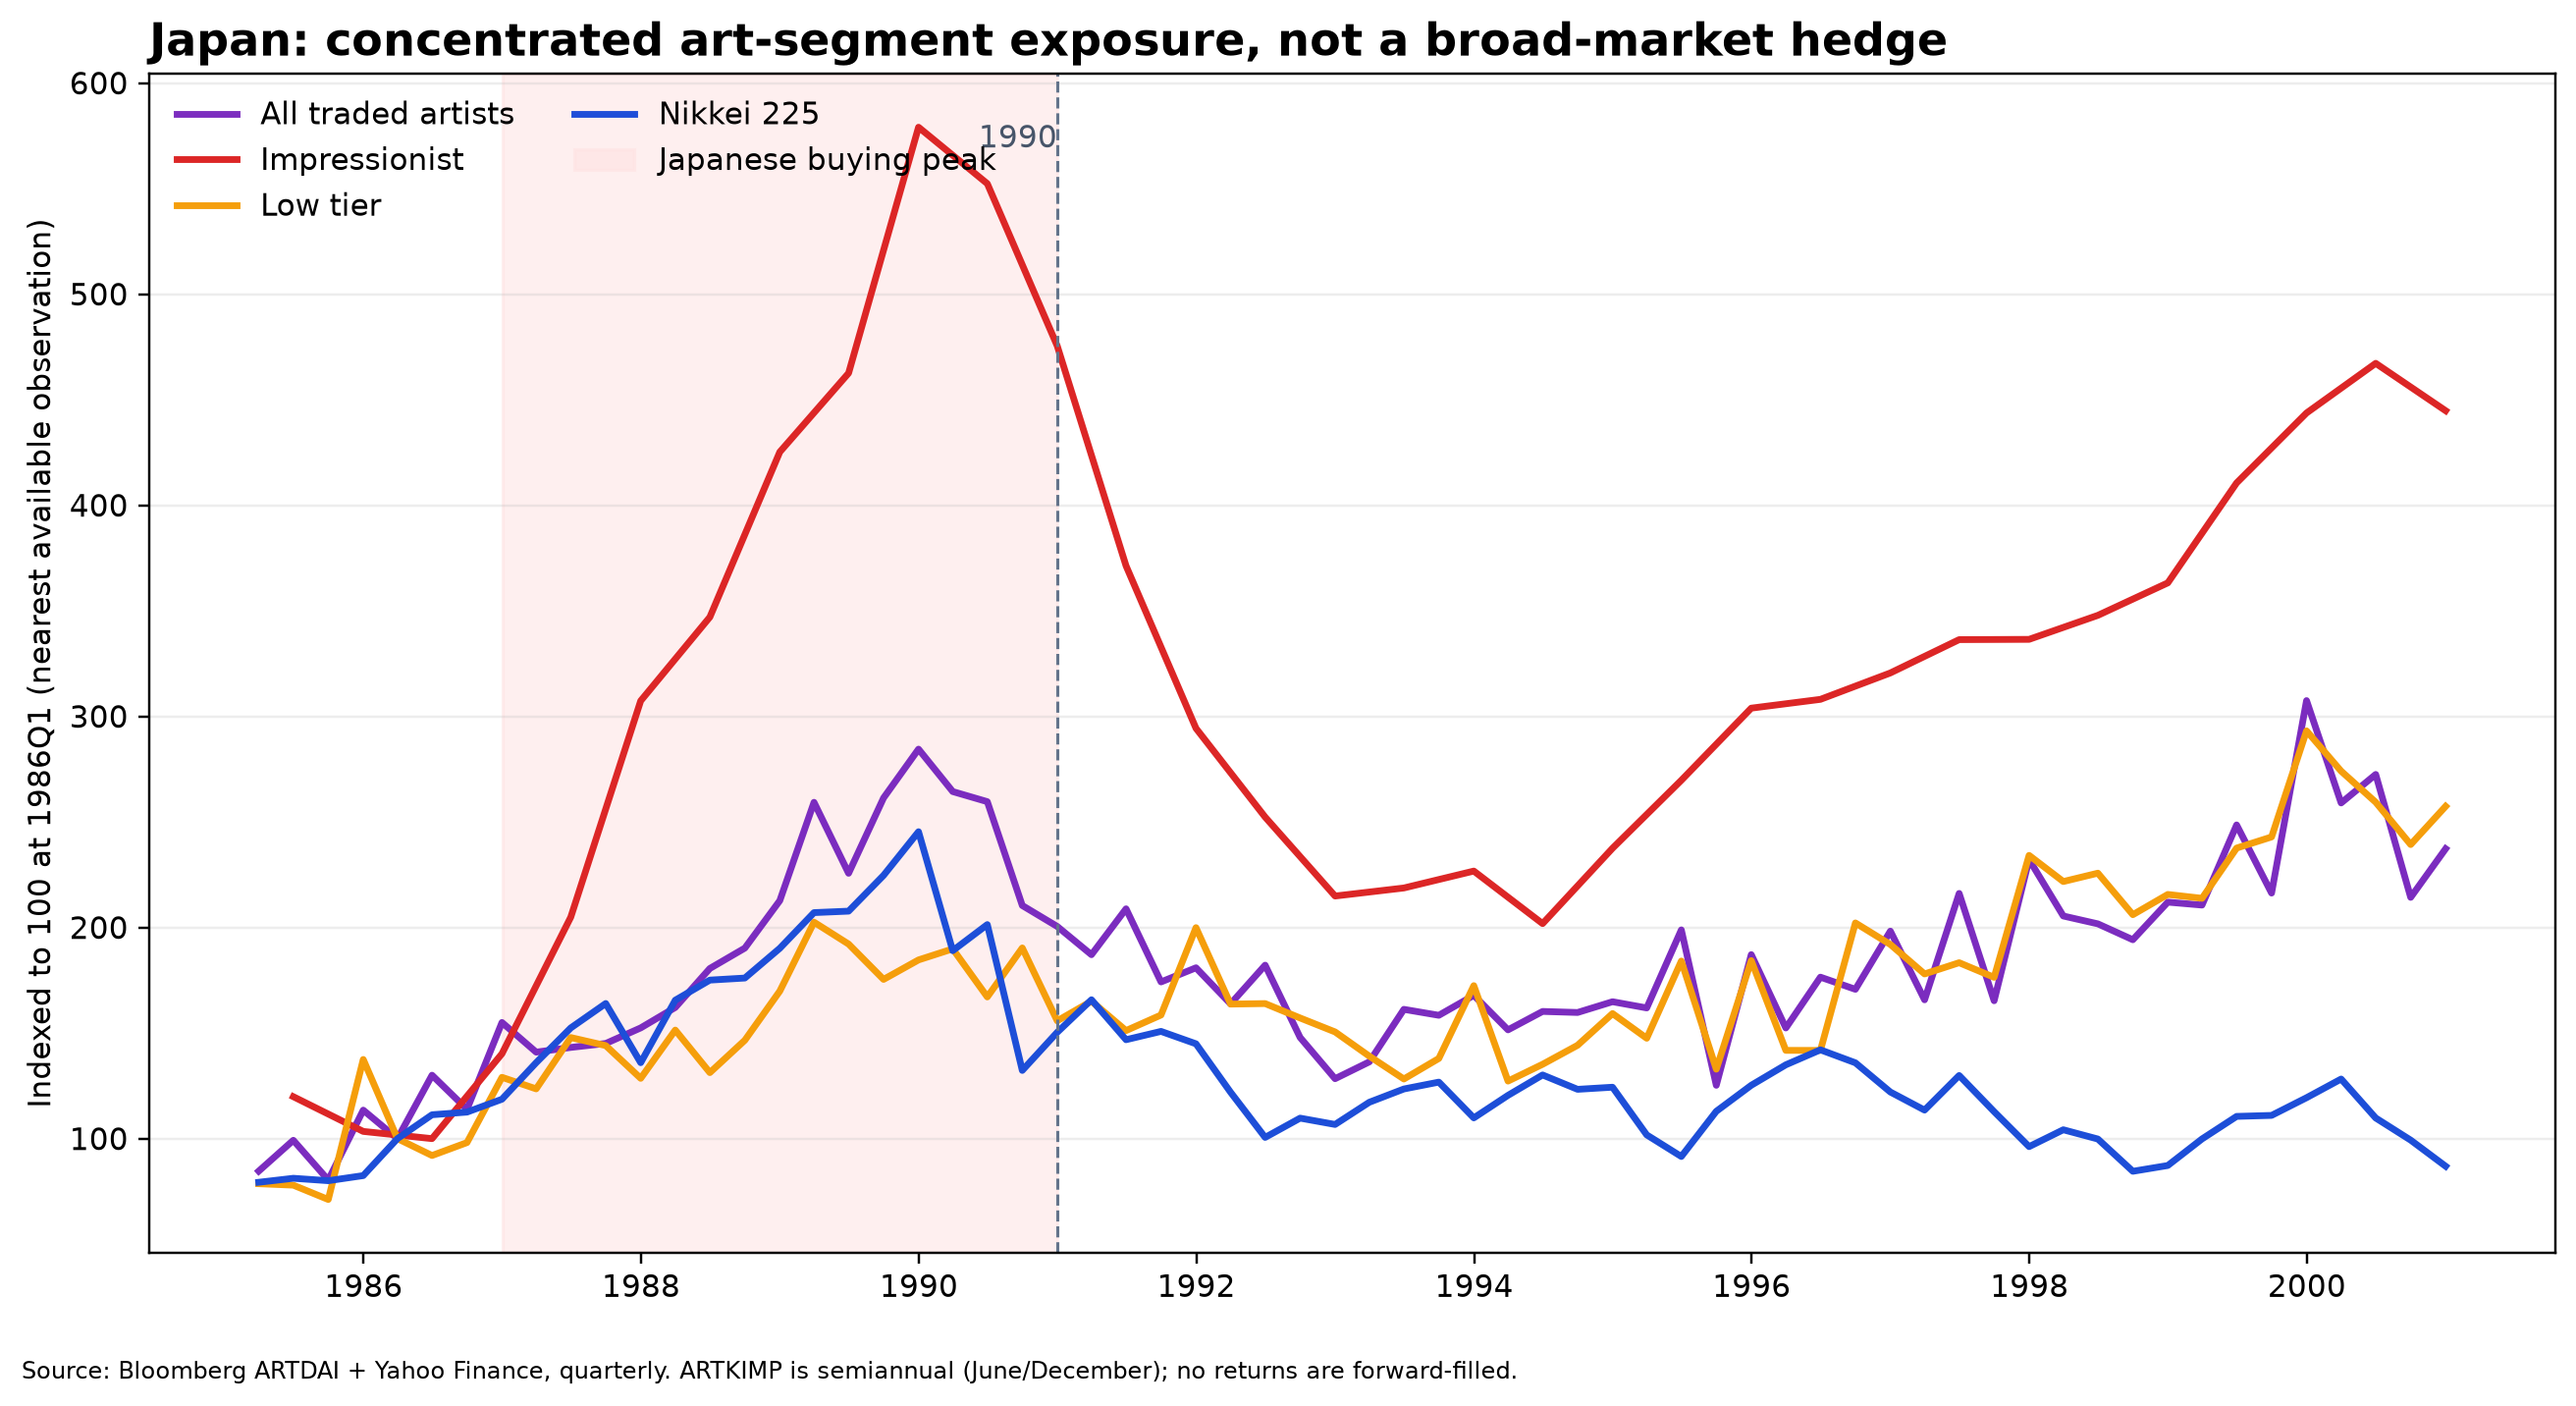
\includegraphics[width=0.70\textwidth]{exhibits/ex4_japan_bubble.png}
\caption{The Japanese asset bubble as a crowded trade: Impressionist art vs.\ the Nikkei. The crash
scaled with prestige (broad $-56\%$, Impressionist $-65\%$, Tier One $-88\%$).}
\end{figure}

\begin{figure}[h]\centering
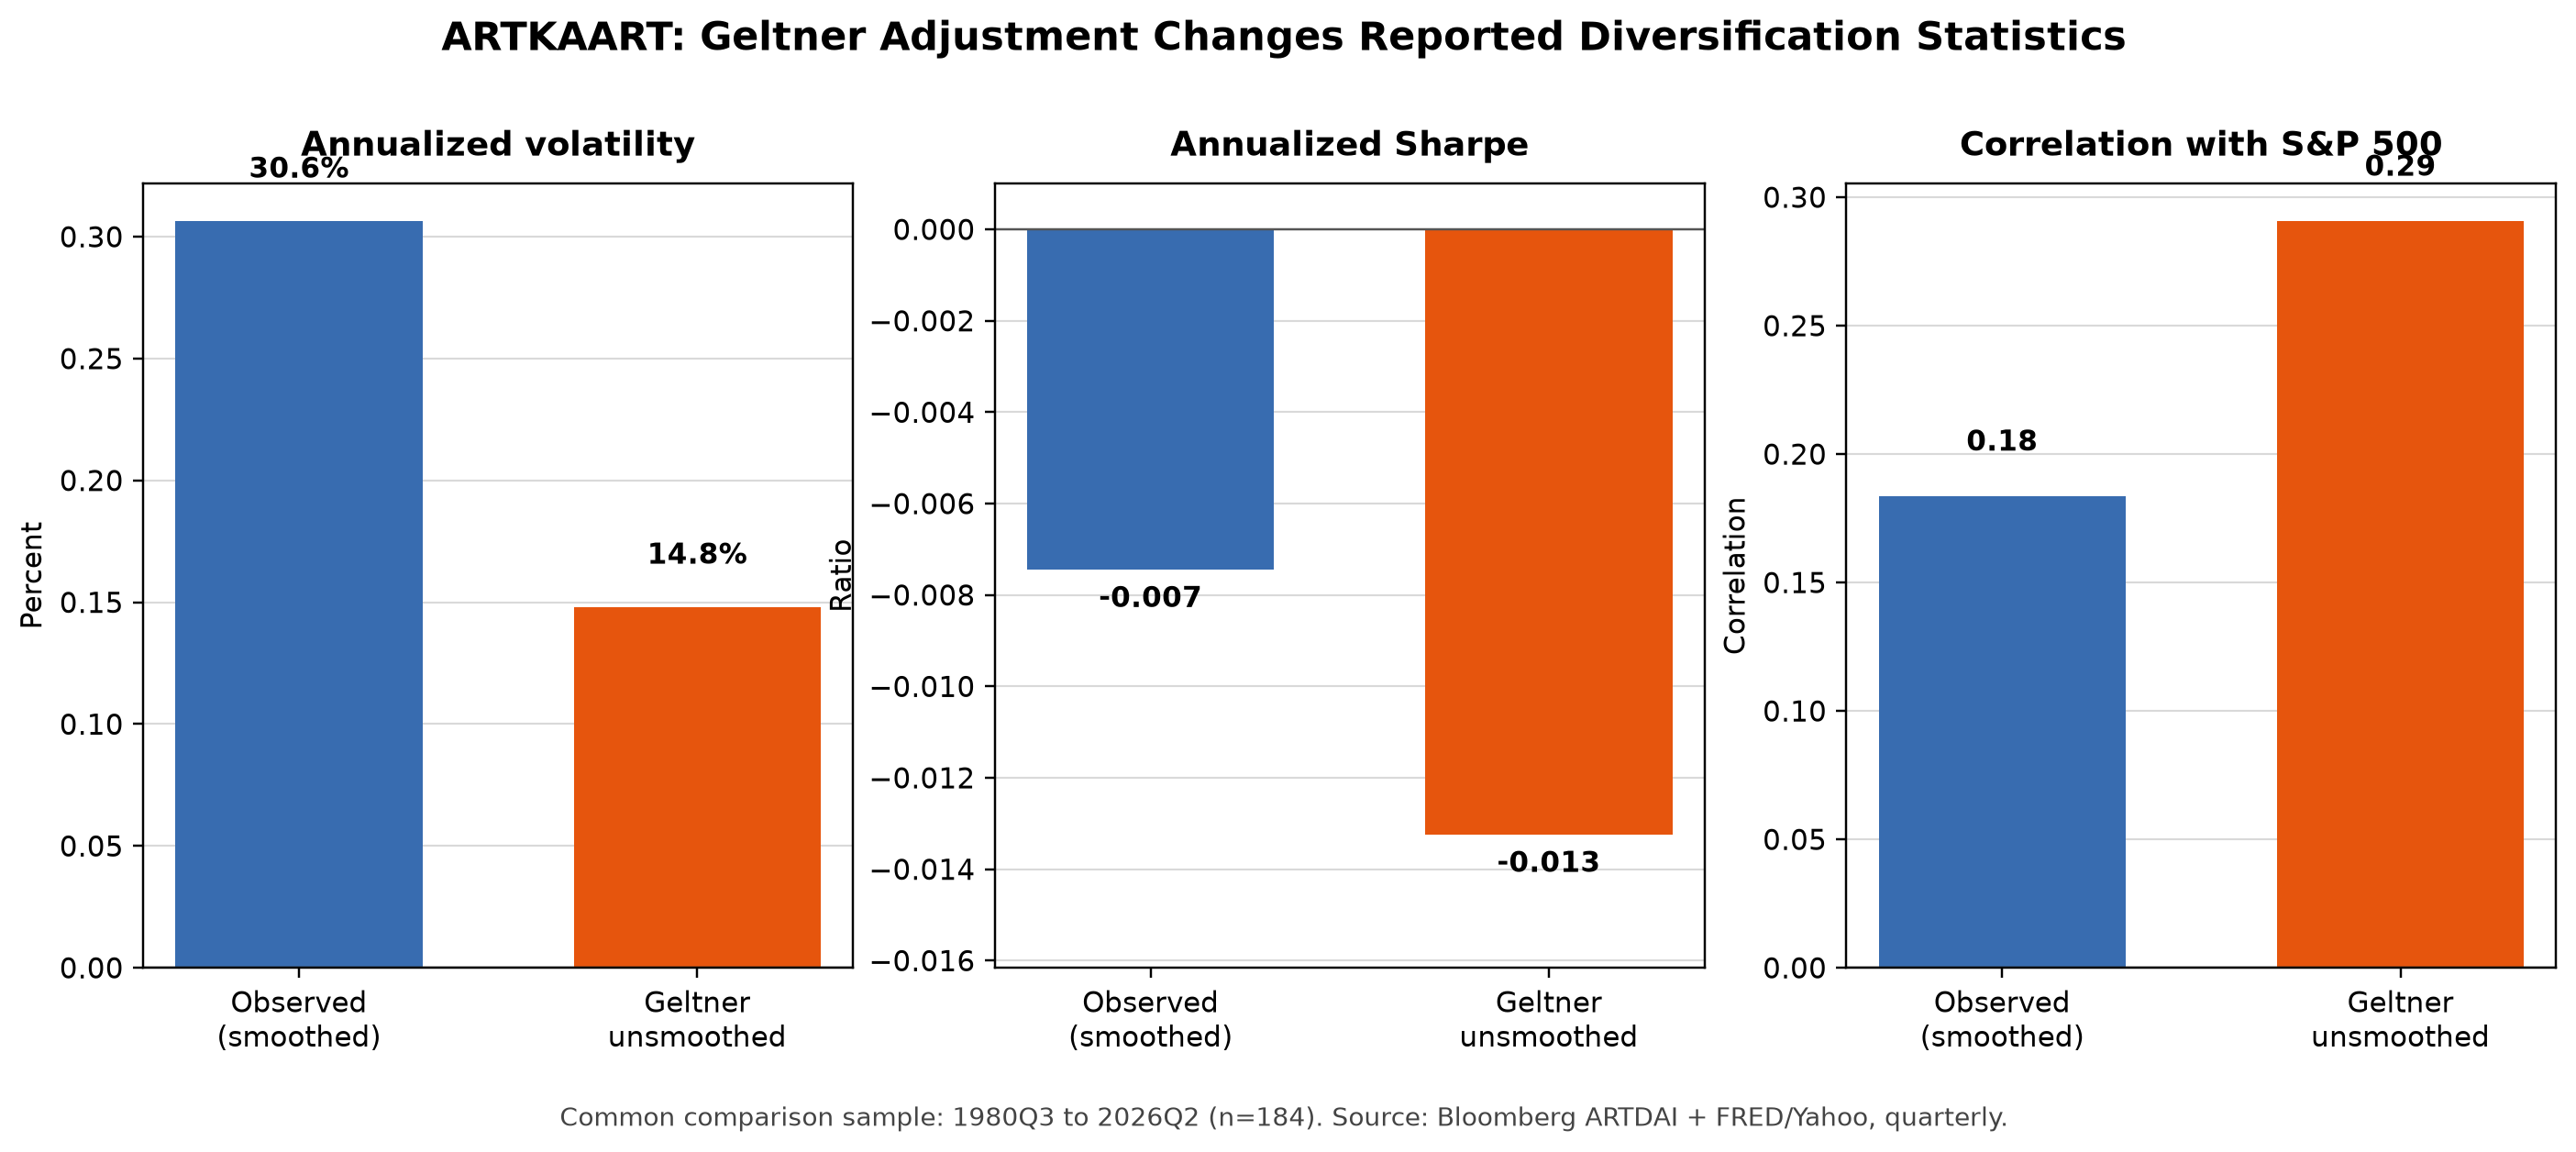
\includegraphics[width=0.66\textwidth]{exhibits/ex5_desmoothing.png}
\caption{Smoothed vs.\ desmoothed art risk. Volatility is high either way and the equity correlation
rises after correction; there is no hidden low-risk premium. Source: Bloomberg ARTDAI, Geltner method.}
\end{figure}

\end{document}
